\documentclass[a4paper, 11pt, notitlepage, english]{article}

\usepackage{babel}
\usepackage[utf8]{inputenc}
\usepackage[T1]{fontenc, url}
\usepackage{textcomp}
\usepackage{amsmath, amssymb}
\usepackage{amsbsy, amsfonts}
\usepackage{graphicx, color}
\usepackage{parskip}
\usepackage{framed}
\usepackage{amsmath}
\usepackage{xcolor}
\usepackage{multicol}
\usepackage{url}
\usepackage{flafter}
\usepackage{caption}

%\DeclareCaptionLabelSeparator{colon}{. }
\renewcommand{\captionfont}{\sffamily}
\renewcommand{\captionlabelfont}{\bf\sffamily}
\setlength{\captionmargin}{40pt}

\usepackage{geometry}
\geometry{headheight=0.01mm}
\geometry{top=24mm, bottom=29mm, left=39mm, right=39mm}

\renewcommand{\arraystretch}{2}
\setlength{\tabcolsep}{10pt}
\makeatletter
\renewcommand*\env@matrix[1][*\c@MaxMatrixCols c]{%
  \hskip -\arraycolsep
  \let\@ifnextchar\new@ifnextchar
  \array{#1}}
%
% Parametere for inkludering av kode fra fil
%
\usepackage{listings}

\definecolor{javared}{rgb}{0.6,0,0} % for strings
\definecolor{javagreen}{rgb}{0.25,0.5,0.35} % comments
\definecolor{javapurple}{rgb}{0.5,0,0.35} % keywords
\definecolor{javadocblue}{rgb}{0.25,0.35,0.75} % javadoc

\lstset{language=python,
basicstyle=\ttfamily\scriptsize,
keywordstyle=\color{javapurple},%\bfseries,
stringstyle=\color{javared},
commentstyle=\color{javagreen},
morecomment=[s][\color{javadocblue}]{/**}{*/},
% numbers=left,
% numberstyle=\tiny\color{black},
stepnumber=2,
numbersep=10pt,
tabsize=4,
showspaces=false,
captionpos=b,
showstringspaces=false,
frame= single,
breaklines=true}

%
% Definering av egne kommandoer og miljøer
%
\newcommand{\dd}[1]{\ \text{d}#1}
\newcommand{\f}[2]{\frac{#1}{#2}} 
\newcommand{\beq}{\begin{equation}}
\newcommand{\eeq}{\end{equation}}
\newcommand{\bra}[1]{\langle #1|}
\newcommand{\ket}[1]{|#1 \rangle}
\newcommand{\braket}[2]{\langle #1 | #2 \rangle}
\newcommand{\braup}[1]{\langle #1 \left|\uparrow\rangle\right.}
\newcommand{\bradown}[1]{\langle #1 \left|\downarrow\rangle\right.}
\newcommand{\av}[1]{\left| #1 \right|}
\newcommand{\op}[1]{\hat{#1}}
\newcommand{\braopket}[3]{\langle #1 | {#2} | #3 \rangle}
\newcommand{\ketbra}[2]{\ket{#1}\bra{#2}}
\newcommand{\pp}[1]{\frac{\partial}{\partial #1}}
\newcommand{\ppn}[1]{\frac{\partial^2}{\partial #1^2}}
\newcommand{\up}{\left|\uparrow\rangle\right.}
\newcommand{\upup}{\left|\uparrow\uparrow\rangle\right.}
\newcommand{\down}{\left|\downarrow\rangle\right.}
\newcommand{\downdown}{\left|\downarrow\downarrow\rangle\right.}
\newcommand{\updown}{\left|\uparrow\downarrow\rangle\right.}
\newcommand{\downup}{\left|\downarrow\uparrow\rangle\right.}
\newcommand{\bupup}{\left.\langle\uparrow\uparrow\right|}
\newcommand{\bdowndown}{\left.\langle\downarrow\downarrow\right|}
\newcommand{\bupdown}{\left.\langle\uparrow\downarrow\right|}
\newcommand{\bdownup}{\left.\langle\downarrow\uparrow\right|}
\renewcommand{\d}{{\rm d}}
\newcommand{\Res}[2]{{\rm Res}(#1;#2)}
\newcommand{\To}{\quad\Rightarrow\quad}
\newcommand{\eps}{\epsilon}
\newcommand{\inner}[2]{\langle #1 , #2 \rangle}


\newcommand{\bt}[1]{\boldsymbol{#1}}
\newcommand{\mat}[1]{\textsf{\textbf{#1}}}
\newcommand{\I}{\boldsymbol{\mathcal{I}}}
\newcommand{\p}{\partial}
%
% Navn og tittel
%
\author{Jonas van den Brink \\ \texttt{j.v.d.brink@fys.uio.no}}
\title{MAT-INF3360 \\ Mandatory Exercises 2}

\begin{document}
% \maketitle
\section*{Project 3.1}
We look at a system of ODEs on the form
\begin{equation}
\bt{v}_t = \mat{A} \bt{v}(t), \qquad \bt{v}(0) = \bt{v}^0, \label{eq:ODE}
\end{equation}
where $\mat{A} \in \mathbb{R}^{n\times n}$ and $\bt{v}^0 \in \mathbb{R}^n$ are given.

\subsection*{a)}
We let $\mu \in \mathbb{R}$ be an eigenvalue of $\mat{A}$, with corresponding eigenvector $\bt{w} \in \mathbb{R}^n$. We will verify that
$$\bt{v}(t) = e^{\mu t}\bt{w},$$
satisfies (\ref{eq:ODE}) with initial condition $\bt{v}^0 = \bt{w}$.

First we find $\bt{v}_t$:
$$\bt{v}_t = \frac{\d}{\d t}\bt{v}(t) = \frac{\d}{\d t}e^{\mu t}\bt{w} = \mu e^{\mu t} \bt{w} = \mu\bt{v}.$$
Using this we check that the matrix equation is satisfied:
$$\mat{A}\bt{v} = \mat{A}e^{\mu t}\bt{w} = e^{\mu t}\mat{A}\bt{w} = e^{\mu t}\mu \bt{w} = \mu e^{\mu t}\bt{w} = \mu \bt{v} = \bt{v}_t.$$
And we check the initial condition:
$$\bt{v}^0 = \bt{v}(0) = e^{0}\bt{w} = \bt{w}.$$

\subsection*{b)}
We now assume $\mu_1, \mu_2, \ldots, \mu_n$ are $n$ distinct eigenvalues of $\mat{A}$ with corresponding eigenvectors $\bt{w}_1, \bt{w}_2, \ldots \bt{w}_n$. And we will check that the function
$$v(t)  = \sum_{k=1}^n c_k e^{\mu_k t} \bt{\omega}_k,$$
is a solution of (\ref{eq:ODE}) for any coefficients $c_1, c_2, \ldots, c_n \in \mathbb{R}$, with initial vector
$$v^0 = \sum_{k=1}^m c_k \bt{\omega}_k.$$

Again, we start by finding $\bt{v}_t$:
$$\bt{v}_t = \frac{\d}{\d t}\bt{v}(t) = \sum_{k=1}^n c_k \frac{\d}{\d t}e^{\mu_k t}\bt{w}_k = \sum_{k=1}^n c_k \mu_k e^{\mu_k t} \bt{w}_k.$$
Note that unlike the previous case, $\bt{v}_t$ is \emph{not} an eigenvector itself. We now check that the matrix equation is fulfilled
$$\mat{A}\bt{v}(t) = \mat{A}\sum_{k=1}^n c_k e^{\mu_k t} \bt{\omega}_k = \sum_{k=1}^n c_k e^{\mu_k t} \mat{A}\bt{\omega}_k = \sum_{k=1}^n c_k e^{\mu_k t} \mu_k \bt{\omega}_k = \bt{v}_t.$$
And we also check the initial condition
$$\bt{v}^0 = \bt{v}(0) = \sum_{k=1}^n c_k e^{\mu_k 0} \bt{\omega}_k = \sum_{k=1}^n c_k \bt{\omega}_k \quad \mbox{q.e.d.}$$

\clearpage

\section*{c)}
We just showed that the function and initial condition
\begin{equation}
v(t)  = \sum_{k=1}^n c_k e^{\mu_k t} \bt{\omega}_k, \qquad v^0 = \sum_{k=1}^n c_k \bt{\omega}_k. \label{eq:form}
\end{equation}
is a solution to (\ref{eq:ODE}). We will now argue that in fact \emph{all} solutions of the system of ODEs admits this form, when $\mu_1, \mu_2, \ldots, \mu_n$ are the eigenvalues of $\mat{A}$.

When we know that $\mat{A}$ har $n$ distinct eigenvalues, we know that 
the corresponding $n$ eigenvectors $\{\bt{\omega}_k\}$ are non-zero 
and linearily independant. This means that the eigenvectors are a 
basis that span $\mathbb{R}^n$, it is there for readily apparent that 
any initial vector $\bt{v}^0$ can be expressed as
$$\bt{v}^0 = \sum_k c_k \bt{\omega}_k.$$
We have already shown that
\begin{equation}
v(t)  = \sum_{k=1}^n c_k e^{\mu_k t} \bt{\omega}_k, \qquad v^0 = \sum_{k=1}^n c_k \bt{\omega}_k.
\end{equation}
is a solution of (\ref{eq:ODE}) with this initial condition. As we know the eigenvectors are linearily independant, the coefficients $\{c_k\}_{k=1}^n$, give $n$ degrees of freedom---it then readily follows that any solution can be written on the form (\ref{eq:form}).

\subsection*{The Heat Equation}

We now look at the heat equation with Dirichlet boundary conditions
\begin{align}
u_t &= u_{xx}, \quad x\in(0,1), \quad t>0, \\
u(0,t) &= u(1,t) = 0, \\
u(x,0) &= f(x), \quad x\in(0,1).
\end{align}
We can write it using the same operator notation we used in our last project, meaning $Lu = -u_{xx}$. The problem can then be written
\begin{align*}
u_t(x,t) &= -(Lu)(x,t) \quad \mbox{ for } \quad x\in(0,1), \quad t>0, \\ 
u(x,0) &= f(x).    
\end{align*}

We now approximate the problem by discretizing in the spatial dimension. We introduce a uniform mesh with $n$ internal mesh points, and let $x_j = jh$, where $h=1/(n+1)$, so $x_0 = 0$ and $x_{n+1} = 1$ are the boundaries. We use a 2.\ order centeral finite difference approximation to approximate $(-Lu)(x,t)$. To derive a numerical scheme, we now evaluate our PDE in an internal mesh point $x_j$:
$$[v_t(x,t) = -(Lu)(x,t)]_j \approx [v_t = D_x D_x u]_j,$$
which gives
$$v^j_t = \frac{v_{j+1} - 2v_j + v_{j-1}}{h^2}.$$
where $v^j_t$ is shorthand for $v_t(x_j, t)$. This equation holds for all internal mesh points, i.e., for $j=1,2,\ldots, n$. Remember that $v_0 = v_{n+1} = 0.$

\section*{d)}
We now let $n=2$, and will show that the numerical scheme we derived leads to a system of ODE on the form of (\ref{eq:ODE}). From our numerical scheme, we then have the two equations
\begin{align*}
v_t^1 &= \frac{1}{h^2}\big(v_2 - 2v_1 + v_0 \big), \\
v_t^2 &= \frac{1}{h^2}\big(v_3 - 2v_2 + v_1 \big),
\end{align*}
using that $h=1/(n+1) = 1/3$ and $v_0 = v_3 = 0$, we get
\begin{align*}
v_t^1 &= -9\big(2v_1 -v_2 \big), \\
v_t^2 &= -9\big(-v_1 + 2v_2 \big). 
\end{align*}
Which can be written more compactly as a matrix equation
$$\bt{v}_t = \mat{A}\bt{v},$$
where
$$ \mat{A} = -9\begin{pmatrix} 2 & -1 \\ -1 & 2 \end{pmatrix} \mbox{ q.e.d.} $$

\subsection*{e)}
We now let
$$f(x) = \sin(\pi x) - 3\sin(2\pi x),$$
and will find the solution to our semi-descreete problem with $n=2$. First we note that
$$\bt{v}^0 = \begin{pmatrix} v(x_1,0) \\ v(x_2,0) \end{pmatrix} = \begin{pmatrix} f(x_1) \\ f(x_2) \end{pmatrix} = \begin{pmatrix}
    -\sqrt{3} \\ 2\sqrt{3}  
\end{pmatrix},$$
where $x_1 = 1/3$ and $x_2 = 2/3$.

We find the eigenvalues of $$\mat{A}$$ to be $\mu_1 = -9$ and $\mu_2 = -27$ with the corresponding eigenvectors
$$\bt{\omega}_1 = \begin{pmatrix} 1\\ -1 \end{pmatrix} \qquad \bt{\omega}_2 = \begin{pmatrix} 1\\ 1 \end{pmatrix} .$$
We then see that
$$\bt{v}^0 = -\frac{3\sqrt{3}}{2} \bt{\omega}_1 + \frac{\sqrt{3}}{2}\bt{\omega}_2,$$
so the coefficients are $c_1 = -3\sqrt{3}/2$ and $c_2 = \sqrt{3}/2$, and the solution is
$$\bt{v}(t) = \frac{\sqrt{3}}{2}e^{-27t}\bt{\omega}_2 - \frac{3\sqrt{3}}{2}e^{-9t}\bt{\omega}_1.$$

\clearpage

\subsection*{f)}
We will now show that for all values of $n$, we end up with a system of ODEs on the form (\ref{eq:ODE}) and will identify the matrix $\mat{A}$.

With $n$ internal mesh points, we get the $n$ equations:
$$v^j_t = \frac{v_{j+1} - 2v_j + v_{j-1}}{h^2} \qquad j=0,1,\ldots,n.$$
If we use the fact that $v_0 = v_{n+1} = 0$, we can write these equations as the matrix equation
$$\bt{v}_t = \mat{A}\bt{v},$$
where $\bt{v}_t, v \in \mathbb{R}^n$ and $\mat{A}\in \mathbb{R}^{n\times n}$. We then see that $\mat{A}$ becomes the tridiagonal matrix
$$\mat{A} = -\frac{1}{h^2}\begin{pmatrix}
    2 & -1 & 0 & 0 & \ldots & 0 \\
    -1 & 2 & -1 & 0 &\ldots & 0 \\
    0 & -1 & 2 & -1 & \ldots & 0 \\
    \vdots & \vdots & \ddots & \ddots & \ddots & \vdots \\
    0 & 0 & \ldots & -1 & 2 & -1 \\
    0 & 0 & \ldots & 0 & -1 & 2
\end{pmatrix}. $$
Which can be solved effectively using the Thomas' algorithm, which scales linear with $n$, i.e., $\mathcal{O}(n)$.

\subsection*{g)}
From section 2.4.2, p.\ 68 in \emph{Introduction to Partial Differential Equations} by Tveito and Winther, we know that the eigenvalues of $\mat{A}$ are
$$\mu_k = -\frac{4}{h^2}\sin^2(k\pi h/2).$$
This can also be easily shown from the fact that $\mat{A}$ is both tridiagonal and Toeplitz (meaning the elements along all digaonals are constant). Tridiagonal Toeplitz matrices have known eigenvalues\footnote{\url{http://en.wikipedia.org/wiki/Tridiagonal_matrix#Eigenvalues}}. 

The corresponding eigenvectors are
$$\bt{\omega}(x_j) = \sin(k\pi x_j), \quad j=1,2,\ldots,n.$$

The general solution to the problem (\ref{eq:ODE}) could be written
$$\bt{v}(t) = \sum_{k=1}^n c_k e^{\mu_k t} \bt{\omega}_k.$$
If we write this out for a single component of $\bt{v}(t)$, and insert for $\bt{\omega}_k$ we find
$$v(x_j, t) = \sum_{k=1}^n c_k e^{\mu_k t} \sin(k\pi x_j), \quad j=1,2,\ldots,n.$$

\subsection*{h)}
We now consider the initial function
$$f(x) = 3\sin(\pi x) + 5\sin(4\pi x).$$
We will now compare the semidiscrete solution we just found for $n=2,4,6$ to the exact analytic solution.

It is trivial to see that 
$$c_1 = 3, \qquad c_4 = 5.$$
Meaning the analytic solution is
$$u(x,t) = 3e^{-\pi^2 t}\sin(\pi x) + 5e^{-16\pi^2 t}\sin(4\pi x).$$
and the semi-discrete solution is
$$v(x,t) = 3e^{-\mu_1 t}\sin(\pi x) + 5e^{-\mu_4 t}\sin(4\pi x).$$
Where $\mu_1$ and $\mu_4$ depend on $n$. (Note, we earlier defined $\mu_k$ to be negative, now we define them to be positive and include a negative sign in the exponential).

We now notice that the only difference between the analytic solution and the semi-discrete one is in the exponential factor. This means that the solutions will be equal at $t=0$, which of course is reasonable, as they are both equal to the known intial function $f(x)$.

If we compute $\mu_1$ and $\mu_4$ for an increasing number of mesh points $n$, we see that the values seem to converge toward the known analytic values, which is good:

\begin{center}
    \begin{tabular}{c|c|c}
    & $\mu_1$ & $\mu_4$ \\ \hline
    Analytic &  9.87 & 157.91 \\ \hline \hline
    Semi-discrete, $n = 2$ & 9.00 & 27.00 \\ \hline
    Semi-discrete, $n = 4$ & 9.55 & 90.45 \\ \hline
    Semi-discrete, $n = 6$ & 9.71 & 119.81 \\ \hline
    Semi-discrete, $n = 8$ & 9.77 & 133.87 \\ \hline
    Semi-discrete, $n = 16$ & 9.84 & 150.85 \\ \hline
    Semi-discrete, $n = 32$ & 9.86 & 156.01 \\ \hline
        \end{tabular}
\end{center}

We now plot the analytic solution and the semi-discreet solutions for a small time, $t=0.01$, $n=2, 4, 6$. The figure is shown on the next page. We see that as small values of $n$ give a to small $\mu_1$ and $\mu_4$ we see that all of the semi-discrete solutions die out to slow, and so an animation would show that the smallest $n$ take the longest to die out.

\begin{figure}
\centering
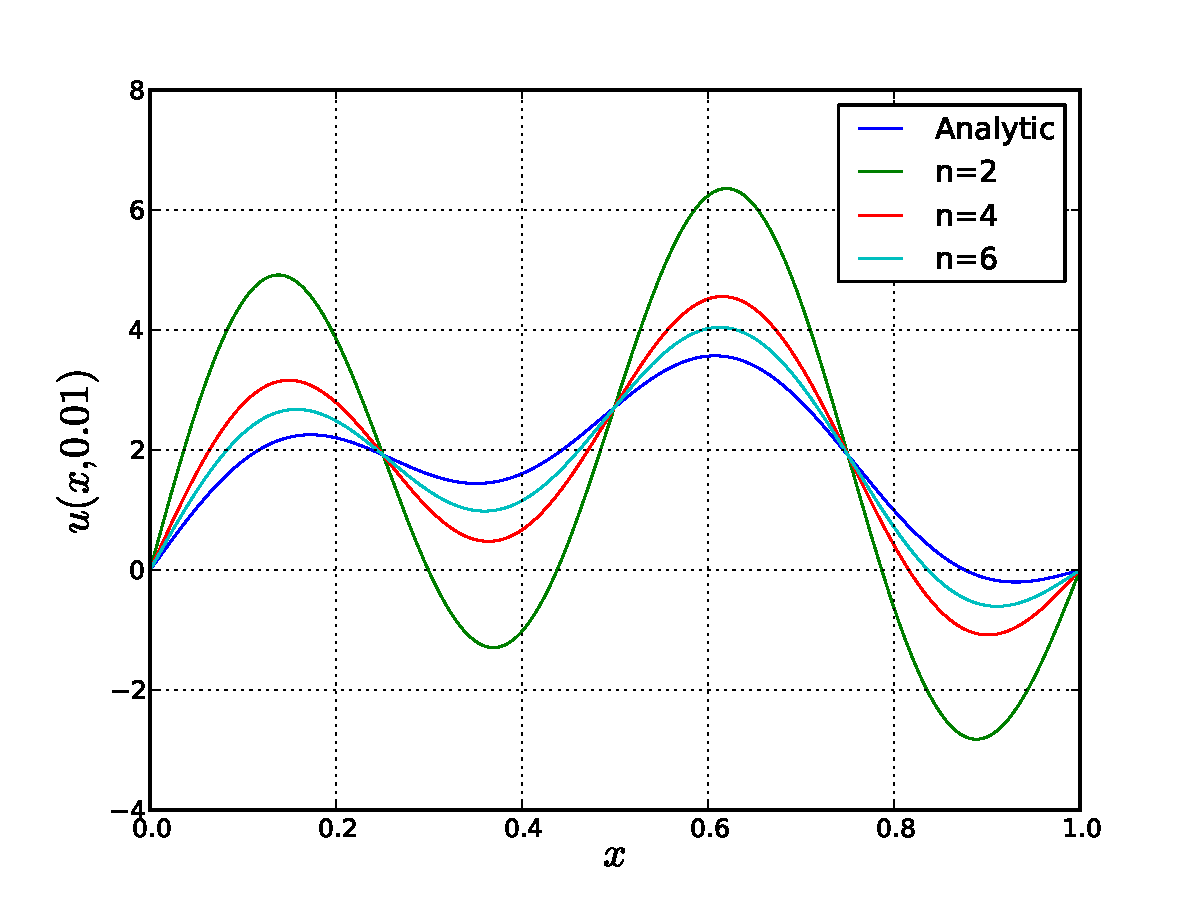
\includegraphics[width=\textwidth]{plot_h.pdf}
\caption{A plot of the known exact solution and semi-discrete solutions for $n=2$, $n=4$ and $n=6$ at time t=0.01. We clearly see that the approximate solutions die out too slowly.}
\end{figure}

\clearpage

\subsection*{i)}

We define the discrete energy of a solution $v$ as
$$E_h(t) = \langle v(x,t), v(x,t) \rangle_h = h\sum_{j=1}^n v(x_j, t)^2 \qquad \mbox{for } t\geq 0.$$
Where we have used that $v_0 = v_{n+1} = 0$.

We will now look at how the discrete energy develops with time, we have
$$\frac{\d}{\d t} E_h(t) = h \sum_{j=1}^n \frac{\d}{\d t} v(x_j, t)^2 = h \sum_{j=1}^n 2v(x_j, t) v_t(x_j, t).$$
We now use the fact that any solution $v$ satisfies
$$v_t(x_j, t) = -(L_h v)(x_j, t),$$
and so we have
$$\frac{\d}{\d t} E_h(t) = -2h\sum_{j=1}^n (L_h v)(x_j, t) v(x_j, t).$$
Or
$$\frac{\d}{\d t} E_h(t) = -2h\langle L_h v, v\rangle.$$
But from Lemma 2 we know that the operator $L_h$ is positive-definite, meaning that for any solution $v$ we know that
$$\langle L_h v, v \rangle \geq 0,$$
where the equality is only true for the trivial solution $v = 0$.

This means that
$$\frac{\d}{\d t} E_h(t) \leq 0,$$
and
$$E_h(t) \leq E_h(0) \qquad \mbox{for } t \geq 0.$$ 
And so we see that any solution of the semi-discrete problem has the same energy decay characteristic as the analytic solution.

\subsection*{j)}
We will now obtain a fully discrete finite difference method by applying a forward difference to the time-derivative. This means we get an explicit forward Euler scheme for the heat equation. We use a uniform mesh in both dimensions, and sample our PDE in the points $t_m$
and $x_j$:
$$\big[D_t v(x, t) = [D_x D_x v(x, t)\big]^m_j,$$
writing out the finite difference operators gives
$$\frac{v_j^{m+1}-v_j^m}{\Delta t} = \frac{v_{j+1}^t - 2v_j^t + v_{j-1}^t}{h^2},$$
solving for $v_j^{m+1}$ gives the numerical scheme
$$v_j^{m+1} = v_j^m + \frac{\Delta t}{h^2}\big(v_{j+1}^t - 2v_j^t + v_{j-1}^t\big) \mbox{ for } m=0,1,2,\ldots.$$

Writing the numerical scheme out for $j=1,2,\ldots,n$
gives a system of $n$ linear equations, 
which can be written as the matrix equation
 $$\bt{v}^{m+1} = (\mat{I} + \Delta t \mat{A})\bt{v}^m.$$
Where $\mat{A}$ is the same
 matrix as earlier, 
 and $\mat{I}$ is the $n\times n$ identity matrix.

\subsection*{k)}
As $\mat{A}$ is the same as before, we know that it has $n$ distinct eigenvalues $\mu_k$ with corresponding eigenvectors $\bt{\omega}_k$. 

As the $n$ distinct eigenvectors span $\mathbb{R}^n$, we know that we can write the inital vector as
$$\bt{v}^0 = \sum_{k=1}^n c_k \bt{\omega}_k.$$
When calculating $v^1$ we have
$$\bt{v}^1 = (\mat{I} + \Delta t \mat{A})^m \sum_{k=1}^n c_k \bt{\omega}_k = \sum_{k=1}^n c_k \big(\mat{I} \bt{\omega}_k + \Delta t \mat{A}\bt{\omega}_k\big) = \sum_{k=1}^n c_k (1  + \Delta t \mu_k)\bt{\omega}_k.$$
But this process is repeatable, so to find the solution at $t_m$ we just matrix-multiply $m$ times. We then end up with
$$\bt{v}^m = \sum_{k=1}^n c_k (1  + \Delta t \mu_k)^m \bt{\omega}_k.$$
Or if we insert for $\bt{\omega}_k$ and write the solution out in a single mesh point:
$$v(x_j, t_m) = \sum_{k=1}^n c_k (1  + \Delta t \mu_k)^m \sin(k\pi x_j)\qquad \mbox{q.e.d.}$$

\clearpage

\section*{Exercise 4.16}

\subsection*{a)}
We will now use Von Neumann stability analysis to show that the Crank-Nicolson scheme is unconditionally stable.

The numerical scheme is as follows
$$\frac{v_j^{m+1} - v_j^m}{\Delta t} = \frac{1}{2}\bigg(\frac{v_{j+1}^{m+1} - 2v_j^{m+1} + v_{j+1}^{m+1}}{\Delta x^2} + \frac{v_{j+1}^{m} - 2v_j^{m} + v_{j+1}^{m}}{\Delta x^2} \bigg).$$

We now insert a fourier element into this discrete equation, and see how the element grows, for some wave-number $k$ we have 
$$v_j^m = e^{at}e^{ikx},$$
inserting this and dividing by $v_j^m$ gives:
$$e^{a\Delta t} - 1 = \frac{\Delta t}{2\Delta x^2}\big(e^{a\Delta t}+1\big)\big(e^{ik\Delta x} + e^{-ik\Delta x} - 2\big).$$
We now use the fact that:
$$e^{ik\Delta x} + e^{-ik\Delta x} - 2 = 2\cos(k\Delta x) - 2 = -4\sin^2\bigg(\frac{k\Delta x}{2}\bigg).$$
to rewrite this as
$$e^{a\Delta t} - 1 = -2C\big(e^{a\Delta t} + 1\big) \sin^2\bigg(\frac{k\Delta x}{2}\bigg),$$
where $C=\Delta t / \Delta x^2$. Solving for the amplification factor gives
$$A = \bigg|\frac{v_j^{m+1}}{v_j^m}\bigg| = e^{a\Delta t} = \frac{1 - 2C\sin^2({k\Delta x / 2})}{1 + 2C\sin^2({k\Delta x / 2})}.$$
as $\sin^2$ evaluates within $[0,1]$ we see that
$$|A|\leq 1.$$
So the Crank-Nicolson scheme has no growing solutions for any value of $C$.

However, to avoid oscillating solutions, we also have to require that
$$A \geq 0.$$
As the denominator cannot becomen negative, we see that
$$1 - 2C\sin^2(k\Delta x / 2) \geq 0,$$
guarantees that $A \geq 0$. The worst-case here is that $\sin^2$ evaluates to 1, so we have
$$1 - 2C \geq 0,$$
which gives the condition
$$C = \frac{\Delta t}{\Delta x^2} \leq \frac{1}{2}.$$

\clearpage

\subsection*{b)}
The Crank-Nicholson scheme is as follows
$$\frac{v_j^{m+1} - v_j^m}{\Delta t} = \frac{1}{2}\bigg(\frac{v_{j+1}^{m+1} - 2v_j^{m+1} + v_{j+1}^{m+1}}{\Delta x^2} + \frac{v_{j+1}^{m} - 2v_j^{m} + v_{j+1}^{m}}{\Delta x^2} \bigg).$$

\begin{figure}[h]
    \centering 
    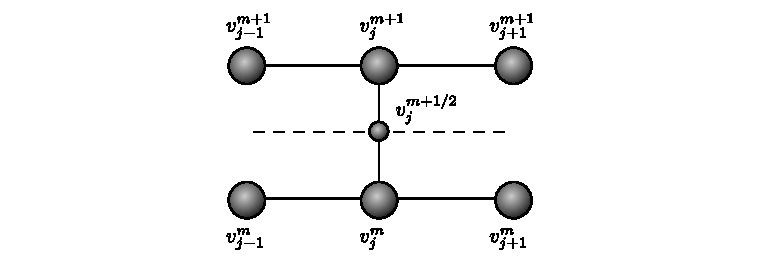
\includegraphics[width=\textwidth]{mol3}
    \caption{Numerical molecule for the Crank-Nicolson scheme.}
\end{figure}

We see that this is in fact an \emph{implicit} scheme, as $\bt{v}^{m+1}$ cannot be explicitly calculated from $\bt{v}^m$, as is the case for the forward Euler scheme. Instead we must solve an algebraic problem, which is in fact a system of linear equation, i.e., a matrix-problem.

To make this more apparent, we rewrite the equation, using $C=\Delta t/\Delta x^2$:
$$-Cv_{j+1}^{m+1} + (2+2C)v_j^{m+1} - Cv_{j-1}^{m+1} = Cv_{j+1}^{m} + (2-2C)v_j^{m} + Cv_{j-1}^{m}$$
Writing out the equations for $j=1,\ldots,n$, we see that this leads to the matrix equation:
$$\mat{A}_+ \bt{v}_{j+1} = \mat{A}_- \bt{v}_{j},$$
where the matrices are both in $\mathbb{R}^{n\times n}$ and have the following elements:
$$ \mat{A}_\pm =
\begin{pmatrix}
2\pm2\alpha & \mp\alpha & \ldots & 0 \\
\mp\alpha & 2\pm2\alpha & \ldots & 0 \\
\vdots & \ddots & \ddots &  \vdots \\
0 & \ldots &  2\pm2\alpha & \mp\alpha \\
0 & \ldots &  \mp\alpha & 2\pm2\alpha 
\end{pmatrix},$$
so both matrices are tridiagonal Toeplitz.

If we simply compute the matrix-vector product on the right as
$$\bt{\tilde{v}}^m = \mat{A}_- \bt{v}^m,$$
we have the matrix-equation
$$\mat{A}_+ \bt{v}^{m+1} = \bt{\tilde{v}}^m.$$
Which is a matrix equation easily solved using the Thomas' algorithm.

\clearpage

\subsection*{c)}
In the last exercise, we showed that the Crank-Nicolson scheme gave rise to the following matrix equation:
$$\mat{A}_+ \bt{v}_{j+1} = \mat{A}_- \bt{v}_{j}.$$
We know that $\mat{A}_+$ is invertible (it is positive definite, which we will show soon), meaning we can left multiply by the inverse of $\mat{A}_+$ to find
$$\bt{v}_{j+1} = \mat{A}_+^{-1}\mat{A}_- \bt{v}_{j}.$$

We can find the eigenvalues/eigenvectors of $\mat{A}_\pm$ by writing them as
$$\mat{A}_\pm = 2\I \pm \Delta t \mat{A}, \qquad \mbox{where }\mat{A} = \frac{1}{\Delta x^2}\begin{pmatrix}
    2 & -1 &  \ldots & 0 \\
    -1 & 2 & \ldots & 0 \\
    \vdots &  \ddots & \ddots & \vdots \\    0 & \ldots & -1 & 2
\end{pmatrix}. $$ 

We know that $\mat{A}$ has the eigenvalues $\mu_k$ and corresponding eigenvectors 
$$\bt{\omega}_j^k = \sin(k\pi x_j), \quad j=1,2,\ldots,n.$$
This means that
$$(2\I \pm \Delta t\mat{A})\bt{\omega}_k = 2\I\bt{\omega}_k \pm \Delta t\mat{A}\bt{\omega}_k = (2 \pm \Delta t \mu_k)\bt{\omega}_k.$$
So we see that $\bt{\omega}_k$ are also eigenvectors for $\mat{A}_\pm$, with eigenvalues $2\pm\Delta t\mu_k$.

From the eigenvalue equation
$$\mat{A}\bt{\omega} = \lambda \bt{\omega},$$
we can find the eigenvalue of an inverse matrix. Assume $\mat{A}$ is invertible, and left-multiply with it:
$$\bt{\omega} = \lambda \mat{A}^{-1} \bt{\omega}.$$
Rearring gives
$$\mat{A}^{-1} \bt{\omega} = \frac{1}{\lambda}\bt{\omega}.$$
So the inverse matrix has the same eigenvector with the reciprocal of the eigenvalue.

Since the eigenvectors $\omega_{k}$ in each case correspond to distinct eigenvalues, we know they are linearily independent, and span $\mathbb{R}^n$, meaning we can expand the inital vector as
$$\bt{v}^0 = \sum_{k=1}^n \gamma_k \bt{w}_k,$$
where the coefficient $\gamma_k$ is found using the inner product with $\bt{v}^0$
$$\gamma_k = \langle \bt{v}^0, \bt{\omega}_k \rangle = \Delta x \sum_{j=1}^n v_j^0 \sin(k\pi x_j).$$

We now have
$$\bt{v}^{1} = \mat{A}_+^{-1}\mat{A}_- \bt{v}_{0},$$
if we insert our expansion of the inital vector
$$\bt{v}^{1} = \sum_{k=1}^n \gamma_k \mat{A}_+^{-1}\mat{A}_- \bt{\omega}_k,$$
which using the fact that $\bt{\omega}_k$ is an eigenvector gives
$$\bt{v}^{1} = \sum_{k=1}^n \gamma_k \frac{2-\Delta t\mu_k}{2+\Delta t\mu_k} \bt{\omega}_k,$$
This process can of course be repeated indefinitely. This means that the solution of the Crank-Nicolson scheme admits the solutions:
$$\bt{v}^m_j = \sum_{k=1}^n \gamma_k a(\mu_k)^m \sin(k\pi x_j),$$
where
$$a(\mu_k) = (2-\Delta t \mu_k)(2 + \Delta t \mu_k)^{-1}.$$

\subsection*{d)}

We will no show that the amplification factor of the Crank-Nicolson scheme is equal to the analytic amplification factor to third order:
$$|a(\mu) - e^{-\mu t}| = \mathcal{O}(\Delta t^3).$$
We insert for $a(\mu)$ and Taylor expand $e^{-\mu t}$:
$$\bigg|\frac{2-\Delta t\mu}{2 + \Delta t\mu} - \big(1 - \Delta t \mu + \frac{1}{2}\Delta t^2 \mu^2 - \frac{1}{6}\Delta t^3 \mu^3 + \mathcal{O}(\Delta t^4) \bigg|.$$
We now expand the Taylor terms into a fraction
$$\bigg|\frac{2-\Delta t\mu}{2 + \Delta t\mu} - \frac{2-\Delta t \mu  + \frac{1}{2}\Delta t^3 \mu^3 - \frac{1}{3}\Delta t^3 \mu^3 + \frac{1}{12}\Delta t^4 \mu^4}{2+\Delta t \mu} + \mathcal{O}(\Delta t^4) \bigg|.$$
Adding the fractions together now gives
$$\bigg|\frac{\frac{1}{6}\Delta t^3 \mu^3  + \frac{1}{12}\Delta t^4 \mu^4}{2+\Delta t \mu} + \mathcal{O}(\Delta t^4) \bigg|.$$
Which can be simplified to
$$\bigg|\frac{\frac{1}{12}(2 + \Delta t \mu)\Delta t^3 \mu^3}{2+\Delta t \mu} + \mathcal{O}(\Delta t^4) \bigg| = \bigg|\frac{1}{12}\Delta t^3 \mu^3 + \mathcal{O}(\Delta t^4)\bigg|.$$
So we see that
$$|a(\mu) - e^{-\mu t}| = \mathcal{O}(\Delta t^3),$$
holds and the Crank-Nicolson is of third-order locally, meaning it is second-order globally. We can compare this to both the explicit forward Euler method and the implicit backward Euler method, which both are first-order globally.

\clearpage

\subsection*{e)}
We will now implement the Crank-Nicolson scheme. In exercise b) we outlined the method we will be using for solving the scheme, which resulting in solving the equation
$$\mat{A}_+ \bt{v}^{m+1} = \bt{\tilde{v}}^m, \qquad \bt{\tilde{v}}^m = \mat{A}_- \bt{v}^m.$$
Calculating 
$\bt{\tilde{v}}^m$
 is straight forward.
However, to solve the matrix equation, we will use the Thomas algorithm, so let us outline it.

\subsubsection*{The Thomas Algorithm}
The Thomas algorithm, also known as the tridiagonal matrix algorithm, is a method to solve a matrix equation:
$$\mat{A}\bt{x} = \bt{y},$$
where the vector $\bt{y}$ is known, the matrix $\mat{A}$ is known and tridiagonal and $\bt{x}$ is to be found. We can write the augmented matrix to be solved as
$$ \left(\mat{A} \mid \bt{y} \right) = 
\begin{pmatrix}[ccccc|c]
b_1 & c_1 &  0 &   \ldots & 0 & {y}_1 \\
a_2 &  b_2 & c_2 &  \ldots & 0 & {y}_2\\
\vdots & \ddots &  \ddots & \ddots & \vdots & \vdots\\
0 & \ldots &  a_{n-1} & b_{n-1} & c_{n-1} & y_{n-1}\\
0 & \ldots &  0 & a_n & b_n & y_n
\end{pmatrix},
$$
where $a_i$, $b_i$, $c_i$ and $y_i$ are constants.

To solve the equation we must get the augmented matrix to upper triangular form. This requires only the elementary row operations 
$${\rm row}_{i+1} - \frac{a_{i+1}}{b_i}{\rm row}_i \quad {\rm for} \ i=1,2,\dots,n-1.$$
Due to $\mat{A}$ being tridiagonal, only a few values of row$_{i+1}$ actually needs to be changed, giving
\begin{align*}
a'_{i+1} = 0, \qquad b'_{i+1} = b_{i+1} - \frac{a_{i+1}}{b_i} c_i, \qquad y'_{i+1} = y_{i+1} - \frac{a_{i+1}}{b_i} \tilde{y}_{i}.
\end{align*}
Written in pseudocode, the decomposition can be written
\begin{lstlisting}[frame=single]
for i = 1:(n-1)
  p = a(i+1)/b(i)
  a(i+1) = 0
  b(i+1) -= p*c(i)
  y(i+1) -= p*y(i)
\end{lstlisting}
When the matrix is in upper triangular form, the answer $\bt{x}$ can be found from a simple backward substitution, the pseudocode is
\begin{lstlisting}
x(n) = y(n)/b(n)
for i = (n-1):1
  x(i) = (y(i) - c(i)*x(i+1)) / b(i) 
\end{lstlisting}

\subsubsection*{Implementation}
We now implement the Crank-Nicolson method for our problem in C++:
\begin{lstlisting}[language=c++]
void Crank_Nicolson(double **u, double r, int n, int m) {
    // Dynamic-memory allocation of vectors
    double *b, *v, p;
    b = new double[n+1];
    v = new double[n+1];
    double c = 2 - 2*r;
    b[0] = 2 + 2*r;

    for (int j=1; j<=m; j++)
    {
        // Initialize tri-diag vectors
        for (int i=1; i<=n; i++)
        {
            b[i] = b[0];
            v[i] = r*u[i+1][j-1] + c*u[i][j-1] + r*u[i-1][j-1];
        }   

        // Decomposition of matrix A
        for (int i=1; i<=(n-1); i++)
        {
            p = -r/b[i];    
            b[i+1] += p*r;
            v[i+1] -= p*v[i];
        }

        // Forward substitution
        u[n][j] = v[n]/b[n];
        for (int i=n-1; i>=1; i--)
            u[i][j] = (v[i] + r*u[i+1][j])/b[i];
    }
}
\end{lstlisting}

And our main program is as follows
\begin{lstlisting}
#include <iostream>
#include <cmath>
#include <cstdlib>
#include <iomanip>
#include <fstream>

using namespace std;

void Crank_Nicolson(double **C, double, int, int);

int main(int argc, char* argv[]) {
    if (argc!=2) {
        cout << "Bad usage: " << argv[0] <<
        "Please specify outfile" << endl;
    exit(1);
    }

    // Prepare outfile
    ofstream outfile;
    outfile.open(argv[1], ios::binary);

    int n = 11;
    int m = 250;

    double L = 1; double T = 0.1;
    double x0=0; double t0=0;

    double dx = L/(n+1);
    double dt = T/(m+1);
    double alpha = dt/dx/dx;
    double *x, *t;
    x = new double[n+2];
    t = new double[m+2];
    for (int i=0; i<=n+1; i++)
        x[i] = x0 + i*dx;
    for (int i=0; i<=m+1; i++)
        t[i] = t0 + i*dt;

    // Dynamic-memory allocation of matrix
    double **u;
    u = new double *[n+2];
    for (int i=0; i<=n+1; i++)
        u[i] = new double[m+2];

    // Initial condition
    for (int i=0; i<=n+1; i++) {
        if (x[i] < 0.5)
            u[i][0] = 2*x[i];
        else
            u[i][0] = 2*(1-x[i]);
    }
        
    // Boundry conditions
    for (int j=1; j<=m+1; j++)
        u[0][j] = u[n][j] = 0;

    
    Crank_Nicolson(u, alpha, n, m);

    // Writing results to outfile
    for (int i=0; i<=n+1; i++)
        for (int j=0; j<=m+1; j++)
            outfile.write((char*) &u[i][j], sizeof(double));
    
    outfile.close();
    return 0;
}
\end{lstlisting}

We now try to run our program for different values of $r = \Delta t/\Delta x^2$ to check the stability of the scheme.
We see that for all $r$, even very large ones - the solution dies out over time as expected - there are no growing solutions.
However, we see that when $r > 0.5$, there are small oscillations in the solutions, that should not be there. These oscillations
die out alongside the solution---this is different from the explicit forward Euler schemes where we can have oscillations that grow with time.

We thus see that the Crank-Nicolson scheme is unconditionally stable with respect to $r$ in the sense that it always converges to the correct solution
as time grows. It is however subject to oscillations, which the implicit backward euler method is not.

\end{document} 

